%Preparando documento
% !TeX program = pdflatex
% !TeX spellcheck = es_ES
% !TeX encoding = utf8
\documentclass[10pt,twocolumn,titlepage]{article}


\usepackage[utf8x]{inputenc}
\usepackage[spanish]{babel}
\usepackage[a4paper,top=2cm,bottom=2cm,left=2cm,right=2cm,marginparwidth=1.75cm,headheight=28pt]{geometry}
%No usar a no ser que sea una emergencia!
% \usepackage[no-math]{fontspec}
% \setmainfont{Comic Sans MS}
\usepackage{booktabs}
\usepackage{graphicx}
\usepackage{xcolor}
%Chiches para escribir matematica super linda
\usepackage{siunitx}
\sisetup{
detect-family,
detect-display-math = true, 
output-decimal-marker = {,} %Esto decide si el separador decimal es coma o punto
}
\usepackage{csquotes}
\usepackage{pdfpages}
\usepackage{fontawesome}
%ANIMACIÓN
%\usepackage{chngcntr}
%\usepackage{animate}
%\usepackage{media9}


\usepackage{mathtools}
\usepackage{color}
\usepackage{amsmath}
\usepackage{amssymb}
\usepackage{cancel}
%\usepackage{fourier}%NO USAR
\renewcommand\spanishtablename{Tabla}

%Fuente (Helvetica, Euclid o ltnmdrn para math, re piola el Euclid)
\renewcommand{\familydefault}{\sfdefault}
\usepackage[scaled=1]{helvet}
\usepackage[format=plain,
            labelfont={bf,it},
            textfont=it]{caption}
\usepackage{hyperref}
\hypersetup{
    colorlinks,
    citecolor=black,
    filecolor=black,
    linkcolor=black,
    urlcolor=black
}
% BACKGROUND CARATULA -------
\usepackage[pages=some]{background}

\backgroundsetup{
scale=1.01,
color=black,
opacity=0.6,
angle=0,
position={7.93,-12.21},
contents={%
  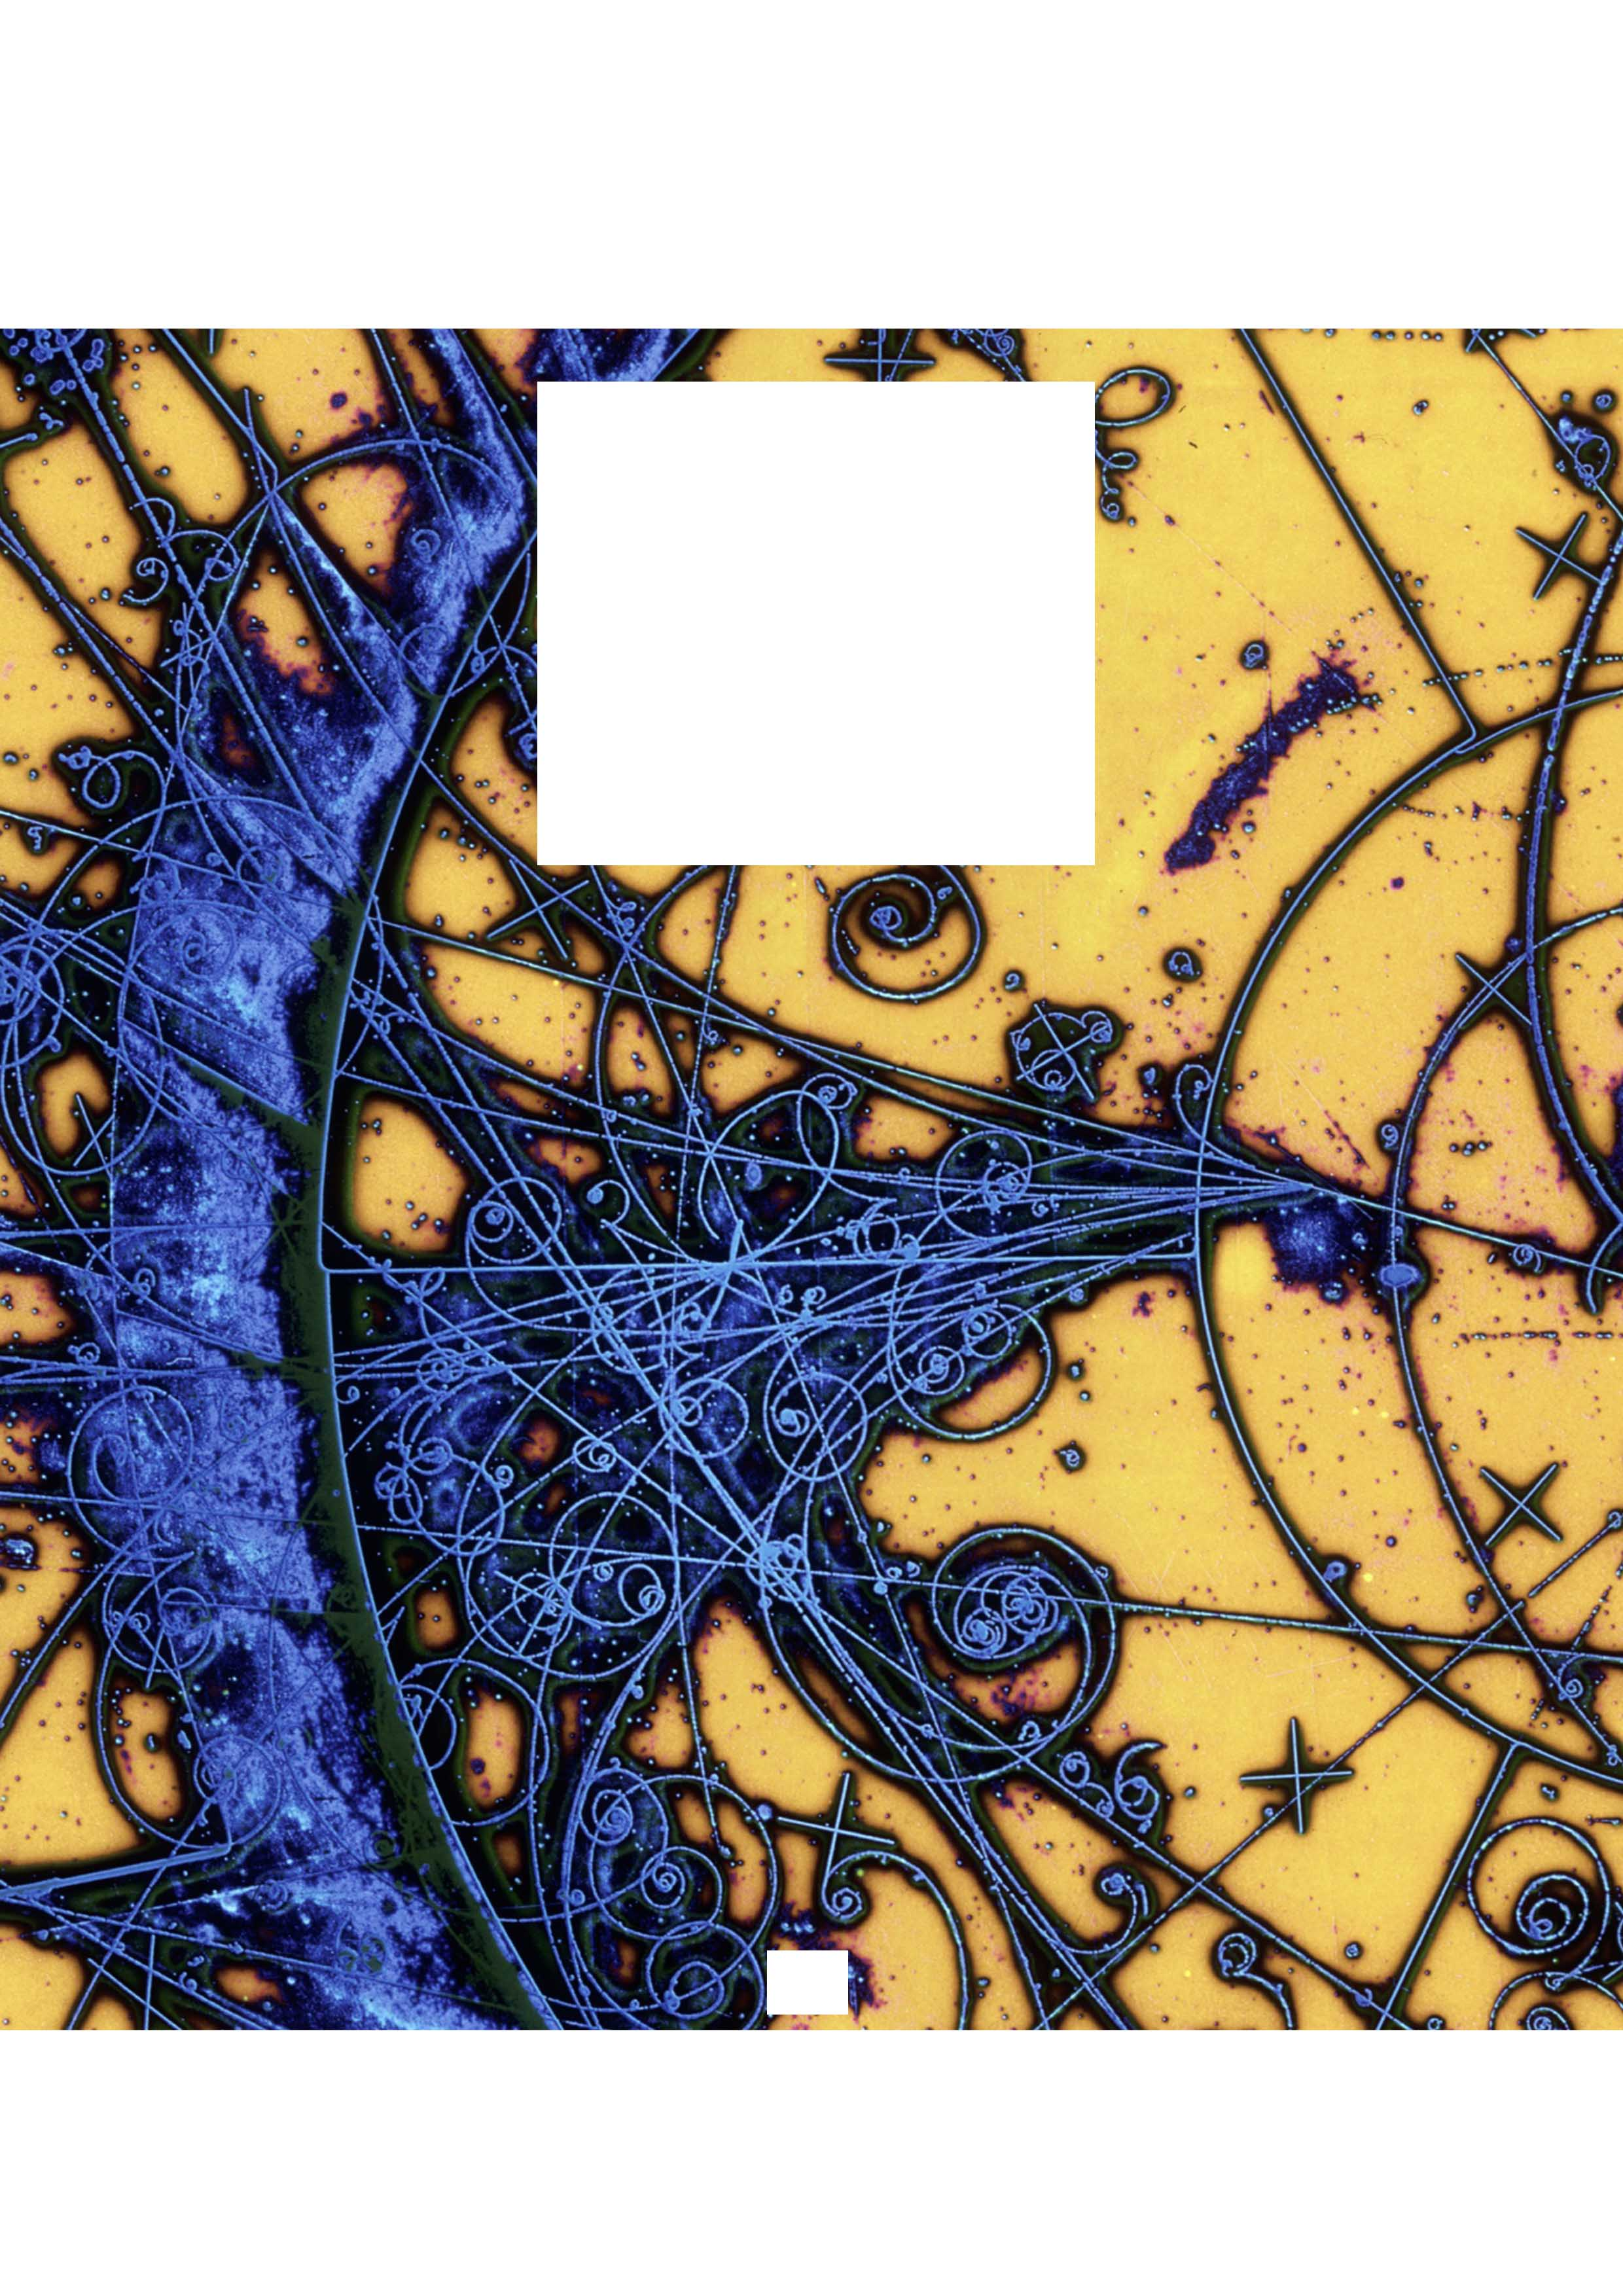
\includegraphics[width=\paperwidth]{Untitled-2.jpg}
  }%
}
%---------------

%TITLE
\title{Carpeta LaTeXeada}

%Comandos customized
%COLORES
\definecolor{dgreen}{RGB}{0, 110, 4}
\definecolor{dblue}{RGB}{16, 53, 112}
%Para usar el simbolo de peligro
\newcommand{\ojo}{\text{\faExclamation}}
\definecolor{verdoso}{RGB}{60, 79, 62}
%
\newcommand\numberthis{\addtocounter{equation}{1}\tag{\theequation}}
\newcommand{\spartial}[2]{\frac{\partial #1}{\partial #2}}
\newcommand{\dpartial}[2]{\frac{\partial^2 #1}{\partial #2^2}}
\newcommand{\uno}{\textrm{I}}
\newcommand{\dos}{\textrm{II}}
\newcommand{\lorenz}{\frac{1}{\sqrt[]{1-\frac{v^2}{c^2}}}}
\newcommand{\Psixt}{\Psi (x,t)}
\newcommand{\psix}{\psi (x)}
%\newcommand{\nabla}{\rotatebox[origin=c]{180}{\Delta}}
\newcommand{\glossentry}[2]{$#1$\indent #2 \par \vspace{.4cm} } %Entradas para glosario
\newcommand{\inpar}[1]{\Bigg( #1 \Bigg)} %PArentheses grandes
\newcommand{\formu}[2]{ #1 $$#2$$ \par \vspace{.4cm} }%Formula
\newcommand{\formuc}[2]{ #1 $$#2$$ } %Formula sin espacio libre al final
\newcommand{\cte}[3]{ $#1$= \SI{#2}{#3} \par \vspace{.4cm} }
\newcommand{\boltz}{k_\textrm{B}}
\newcommand{\lambdadb}{\lambda_{\textrm{DB}}}
\newcommand{\frecdb}{f_{\textrm{DB}}}
\newcommand{\lspeed}{\textit{\textrm{c}}}
\newcommand{\inicial}{\textrm{i}}
\newcommand{\final}{\textrm{f}}
\newcommand{\minima}{\textrm{mín}}
\newcommand{\maxima}{\textrm{máx}}
\newcommand{\Rydberg}{\textrm{R}}
\newcommand{\Avogadros}{\textrm{N}_{\!A}}
\newcommand{\A}{\textrm{A }}
\newcommand{\B}{\textrm{B }}
\newcommand{\atomos}{\acute{a}tomos}
\newcommand{\corr}{\textrm{\color{red} posible error }}
\newcommand{\transm}{\textrm{transm}}
\newcommand{\refl}{\textrm{refl}}
\newcommand{\di}{\,\textrm{d}}
\newcommand{\nucleo}{ {\textrm{núcleo}}}
\newcommand{\atomo}{ {\textrm{átomo}} }
\newcommand{\nqm}{ m_{\iota} }
\newcommand{\nql}{l}
\newcommand{\nqn}{n}

\usepackage{yfonts}
\begin{document}

\begin{titlepage} % Suppresses headers and footers on the title page

% Original titlepage author:
% Peter Wilson (herries.press@earthlink.net) with modifications by:
% Vel (vel@latextemplates.com)
%
% License:
% CC BY-NC-SA 3.0 (http://creativecommons.org/licenses/by-nc-sa/3.0/)


    \fontfamily{fourierenc}\selectfont %Elijo una fuente
    \BgThispage
    
    
	\centering % Centre everything on the title page
	
	%------------------------------------------------
	%	Top rules
	%------------------------------------------------
	
	\rule{\textwidth}{1pt} % Thick horizontal rule
	
	\vspace{2pt}\vspace{-\baselineskip} % Whitespace between rules
	
	\rule{\textwidth}{0.4pt} % Thin horizontal rule
	
	\vspace{0.1\textheight} % Whitespace between the top rules and title
	
	%------------------------------------------------
% 		Title
	%------------------------------------------------
	
	\textcolor{black}{ % Red font color
		{\Large\scshape De qué hablo cuando hablo de}\\[1.5\baselineskip] % Title line 1
		 % Title line 2
		{\Huge Física Moderna} % Title line 3
	}
	
	\vspace{0.025\textheight} % Whitespace between the title and short horizontal rule
	
	\rule{0.3\textwidth}{0.4pt} % Short horizontal rule under the title
	
	\vspace{0.1\textheight} % Whitespace between the thin horizontal rule and the author name
	
	%------------------------------------------------
	%	Author
	%------------------------------------------------
	
	{\Large \textsc{Física IV -- 93.44}} % Author name
	\vspace{3cm}
    
%     \begin{figure}[htb!]
% \begin{center}
% \animategraphics[autoplay,loop, width=0.5\linewidth]{12}{movie/movie-}{1}{30}
% \end{center}

% \end{figure}

	\vfill % Whitespace between the author name and publisher
	
    
	%------------------------------------------------
	%	Publisher
	%------------------------------------------------
	
	{\large\textcolor{verdoso}{\fbox{$\textgoth{WL}$}}}\\[-3\baselineskip] % Publisher logo

	
	\vspace{0.1\textheight} % Whitespace under the publisher text
	
	%------------------------------------------------
	%	Bottom rules
	%------------------------------------------------
	
	\rule{\textwidth}{0.4pt} % Thin horizontal rule
	
	\vspace{2pt}\vspace{-\baselineskip} % Whitespace between rules
	
	\rule{\textwidth}{1pt} % Thick horizontal rule
	
\end{titlepage}


\section*{\centering Glosario} %Aca empieza el Glosario. Ordenado alfabeticamente, primero letras latinas, ultimo letras griegas.
{
\glossentry{B}{Campo magnético.}
\glossentry{c}{Velocidad de la luz.}
\glossentry{E}{Energía total o campo eléctrico.}
\glossentry{E_b}{Energía de enlace.}
\glossentry{E_{A;Z}}{Energía de enlace a nivel atómico.}
\glossentry{E_0=m_0c^2}{Energía en reposo.}
\glossentry{E_T=K+E_0=\gamma m_0c^2}{Energía total.}
\glossentry{e}{Poder emisivo o carga elemental.}
\glossentry{\vec{F}=\frac{d\vec{p}}{dt}=\frac{dm\vec{u}}{dt}}{Fuerza.}
\glossentry{f,\nu}{Frecuencia.}
\glossentry{f_0}{Frecuencia de corte.}
\glossentry{h=2\pi \hbar}{Constante de Planck.}
\glossentry{J(\lambda,T)}{Función de intensidad espectral.}
\glossentry{j}{Densidad de probabilidad de corriente.}
\glossentry{K}{Energía cinética.}
\glossentry{\boltz}{Constante de Boltzmann.}
\glossentry{\ell}{Longitud.}
\glossentry{\ell_p,\,\ell_0}{Longitud propia}
\glossentry{\nql}{Número cuántico orbital.}
\glossentry{m}{Masa aparente o masa en reposo.}
\glossentry{m_0}{Masa en reposo.}
\glossentry{m_s}{Número cuántico de espín (spin).}
\glossentry{\nqm}{Número cuántico magnético $m$.}
\glossentry{\nqn}{Número cuántico principal.}
\glossentry{\vec{p}=\frac{m_0\vec{v}}{\sqrt[]{1-\frac{v^2}{c^2}}}=\gamma m_0\vec{v}}{Cantidad de movimiento.}
\glossentry{q}{Carga.}
\glossentry{\Rydberg}{Constante de Rydberg.}
\glossentry{U,V}{Energía potencial.}
\glossentry{\vec{u},v}{Velocidad.}
\glossentry{u(\lambda,T)}{Función de distribución de energía.}
\glossentry{Z}{Número Atómico.}
\glossentry{\beta=\frac{v}{c}}{Velocidad relativa a la de la luz.}
\glossentry{\gamma=\lorenz}{Factor de Lorentz.}
\glossentry{\varepsilon}{Emisividad.}
\glossentry{\varepsilon_0}{Permitividad, constante dieléctrica}
\glossentry{\kappa=\frac{1}{4\pi\varepsilon_0}}{Constante de Coulomb.}
\glossentry{\phi}{Función de trabajo.}
\glossentry{\lambda}{Longitud de onda, constante de decaimiento.}
\glossentry{\Psi}{Función de onda.}
\glossentry{\psi}{Función posición.}
\glossentry{\sigma}{Constante Stefan-Boltzmann.}
\glossentry{\Omega}{Universo probabilístico.}

{\tiny Algunas letras pueden tomar diferentes sentidos dependiendo del contexto. Por ejemplo, en este documento se va tener en cuenta que $m$ puede ser masa aparente o masa en reposo mientras que $m_0$ siempre es masa en reposo. Noten que el libro siempre usa $m$ para representar masa en reposo.}
 }
 \section*{Sobre esta obra}

 Documento escrito en \textrm{\LaTeX} usando \href{https://www.overleaf.com}{Overleaf}. La caratula es la foto de portada del album \emph{Is This It} -- The Strokes.\par
 
 \vspace{1cm}
 \begingroup

\fontfamily{pbk}\selectfont
\noindent
 Licencia: \faCreativeCommons~BY-NC-SA 4.0
 \endgroup
 


\clearpage
\onecolumn
\tableofcontents  
\clearpage
\twocolumn

 
 \part{Primer Parcial}
%Invariancia: Independiente del sistema de referencia (de su orientacion o lo que sea)
%Covariancia: Las leyes de la fisica son covariantes, osea que tienen la misma forma en todos los sistemas de referencia.
 
\section{Relatividad Especial}
\subsection{Transformaciones}
\begin{align*}
x&=(x^\prime +vt^\prime)\gamma \\
t &= \bigg( t^\prime +\frac{vx^\prime}{c^2}\bigg) \gamma \\
x^\prime &= ( x-vt)\gamma \\
t^\prime &= \bigg(  t-\frac{vx}{c^2}  \bigg)\gamma \\
\ell &= \frac{\ell_p}{\gamma} \\
m &= \gamma m_0 
\end{align*}
\subsubsection*{Transformación de la velocidad}
Imagine un sistema $S^\prime$ que se mueve a velocidad $v$ en la dirección $x$ respecto un sistema $S$. Sí un objeto tiene velocidad $u^\prime_x=c$ en el sistema $S^\prime$ se tiene un absurdo al calcular la velocidad del objeto en el sistema $S$: $u_x=u^\prime_x+v=c+v\ngeq c\; \ojo$. Un objeto con masa no puede superar la velocidad de la luz (ni alcanzarla, estrictamente hablando) en ningún sistema de referencia!

Nos interesa la velocidad de un objeto en $S$. Tenemos que su velocidad $\vec{u}^\prime$ (arbitraria) respecto el sistema de referencia $S^\prime$ mencionado anteriormente. Se tienen que efectuar los siguientes cálculos
\begin{align*}
u_x&=\frac{u^\prime_x+v}{1+\frac{vu^\prime_x}{c^2}}\\
u_y&=\frac{u_y^\prime \sqrt{1-\frac{v^2}{c^2}}}{1+\frac{vu^\prime_x}{c^2}} \\
u_z&=\frac{u_z^\prime \sqrt{1-\frac{v^2}{c^2}}}{1+\frac{vu^\prime_x}{c^2}} 
\end{align*}
Las inversas
\begin{align*}
u^\prime_x&=\frac{u_x-v}{1-\frac{vu_x}{c}}\\
u^\prime_y&=\frac{u_y\sqrt{1-\frac{v^2}{c^2}}}{1-\frac{vu_x}{c^2}}\\
u^\prime_z&=\frac{u_z\sqrt{1-\frac{v^2}{c^2}}}{1-\frac{vu_x}{c^2}}
\end{align*}

\subsection{Inversión temporal}
Supongamos que ocurren dos eventos, el evento $1$ y el evento $2$. $\Delta x>0$ y $\Delta t>0$ nos dice que primero ocurre el evento 1 y después el evento dos ($t_2-t_1>0$). Para que exista un sistema de referencia en el cual los eventos estén invertidos se tiene que cumplir $\Delta t<0$
$$\Delta t=\left(\Delta t-\frac{v\Delta x}{c^2}\right)\gamma\Rightarrow\Delta t-\frac{v\Delta x}{c^2}<0 $$
por lo tanto se tiene que cumplir $\Delta t<\frac{v\Delta x}{c^2}$. Como la información viaja a $c$ tenemos que la condición para que haya inversión temporal es
$$\Delta t < \frac{\Delta x}{c} $$

\subsection{Efecto Doppler}
Se tienen dos relojes, \A y \B sincronizados en $x_0=0$ y $t_0=0$. \B se mueve sobre el eje $x$ positivo a una velocidad $v$ y emite una señal en $x_\B$, $t_\B$.\par 
$t_\A$ es el tiempo que pasa en \A desde $t_0$ hasta que \B emite la señal. Cuando la señal llega al reloj \A este marca $t_\A^\prime$.   $t_\B^\prime$ es el tiempo que marca el reloj \B cuando se inicia la comparación.
$$t_\B^\prime=\bigg( t_\A -\frac{v}{c^2}vt_\A\bigg) \gamma =\bigg( 1-\frac{v^2}{c^2}\bigg)\gamma t_\A= \frac{t_\A}{\gamma} $$
Debo comparar $t_\A^\prime$ con $t_\B^\prime$.
$$x_\B =(t_\A^\prime  -t_\A )c=vt_\A\rightarrow t_\A^\prime=\bigg( 1+\frac{v}{c}\bigg) t_\A$$
$$\therefore \frac{t_\B^\prime}{t_\A^\prime}=\sqrt[]{\frac{1-\frac{v}{c}}{1+\frac{v}{c}}} $$
Expresión en función de frecuencias:
$$f_\textrm{obs}=f_\textrm{fuente} \;\sqrt[]{\frac{1-\frac{v}{c}}{1+\frac{v}{c}}} $$
 %Interacciones ---------------->
\subsection{Interacciones}


Expresión para una fuerza que actúa colineal a la velocidad, por ejemplo, \emph{un electrón sometido a un campo eléctrico}
$$F_{\parallel}=\frac{\di p}{\di t}=\frac{\di mu}{\di t}=\frac{\di }{\di t}\inpar{\:\frac{m_0u}{\sqrt[]{1-\frac{u^2}{c^2}\:}}}=\frac{m_0}{(1-\beta^2)^{3/2}}\frac{\di u}{\di t}$$
$$F_{\parallel}=\gamma^3m_0a $$


Derivación de energía:
\begin{equation} \label{relatividad:diferencialtrabajo}
\di W=\inpar{\frac{\di m}{\di t}\vec{u}+m\frac{\di \vec{u}}{\di t}}\cdot \vec{u}\di t=u^2\di m+mu\di u
\end{equation}
\begin{align*}
\gamma^2 m^2 &= m_0^2    \\
m^2c^2-m^2u^2&= m_0^2c^2 \\
2mc^2\di m-2mu^2\di m-2m^2u\di u &= 0 
\end{align*}
\begin{equation} \label{relatividad:cosa}
c^2\di m=u^2\di m+mu\di u
\end{equation}

reemplazando \ref{relatividad:cosa} en \ref{relatividad:diferencialtrabajo},
\formuc{Integrando de un punto inicial donde la energía cinetica es cero $u_A=0 \Rightarrow m=m_0$, se tiene que el trabajo $W$ es igual a $K$.}{ W=\int_{m_0}^{m}c^2\di m=mc^2-m_0c^2=K}
{De aquí también se obtiene que $E=\gamma m_0c^2$. Se considera que la energía total es una especie de energía cinetica.
\par \vspace{.3cm}}
\begin{equation} \label{relatividad:energiacuadrada}
E^2=p^2c^2+(m_0c^2)^2
\end{equation}

\ref{relatividad:energiacuadrada} es otra expresión para la energía total. Esta se puede aplicar para partículas sin masa en reposo como los fotones:
\begin{align*}
E &= pc \\
mc^2&=pc \\
m&=\frac{p}{c}
\end{align*}
{En otras palabras, un fotón tiene cantidad de movimiento proporcional a su masa aparente. Si nos adelantamos al la relación de De Broglie:}
$$ \lambda=h/p$$
$$\therefore m=\frac{h}{\lambda c} $$
\formu{Una invariante bajo una transformación de Lorentz:}{E^2-p^2c^2}

\formuc{La energía total permanece constante para un sistema de partículas.}{E_{antes}=E_{despu\acute{e}s}}
$$\sum_{i}^{n_1}\gamma_i m_ic^2\bigg|_{t_1}=\sum_{j}^{n_2}\gamma_j m_jc^2\bigg|_{t_2}$$
{\par \vspace{.5cm}}
\formu{Expresión comúnmente llamada fuerza de Lorentz}{\vec{F}=q\vec{E}+q\vec{u}\times\vec{B}}
\formuc{La energía cinetica de una partícula en reposo de carga $q$ sometida a voltaje $V$.}{K=qV}
De acá sale la unidad \si{\eV}, el \emph{electronvolt}, definido como la energía que tiene un electrón que es acelerado a través de una diferencia de potencial de 1 volt. \SI{1}{\electronvolt}=\SI{1.602e-19}{\joule}. Útil para describir todo tipo de proceso atómico!

%Cuerpos Negros----------------->
\section{Cuerpos Negros}
La ley de Rayleigh-Jeans intenta describir la radiación espectral de un cuerpo negro en \si{\watt \per \meter \cubed}. Note que a medida que $\lambda$ se acerca a longitudes de onda pequeñas $e^{\frac{hc}{\lambda \boltz T}}$ tiende a infinito, un problema que se conoció como la \emph{ultraviolet catastrophe}.
$$J(\lambda,T)_{\textrm{RJ}}=\frac{2\pi c\boltz T}{\lambda^4} \; \left[ \si{\kg \per \second \cubed \per \meter}\right] $$
Derivación:
$$J(\lambda,T)=\frac{c}{4}u(\lambda,T)$$
$$u(\lambda,T)=N(\lambda)\big<E\big>$$
$$ N(\lambda)=\frac{8\pi}{\lambda^4} $$
Rayleigh considera la energía continua: 
$$\big<E\big>_{\textrm{RJ}}=\boltz T $$
En 1900 Planck propone que la energía se puede expresar como una suma de paquetes discretos, o \emph{cuanta} (del latín quanta, cantidades) y llega a la siguiente expresión para el valor medio de la energía:
$$ \big<E\big>=\frac{hc}{\lambda\big(e^{\frac{hc}{\lambda \boltz T}}-1\big)}$$
La intensidad espectral[\si{J.m^{-3}s^{-1}}], o la intensidad de la  radiación emitida por un cuerpo negro viene dada por la ley de Planck:

$$ J(\lambda,T)=\frac{2\pi hc^2}{\lambda^5}\frac{1}{e^{\frac{hc}{\lambda \boltz T}}-1 } $$

$$J(f,T)=\frac{2\pi hf^3}{c^2}\frac{1}{e^{\frac{hf}{ \boltz T}}-1 } $$
Si integramos sobre un intervalo de longitud de onda $[\lambda_L,\lambda_H]$ obtenemos el poder emisivo [\si{\watt \per \meter \squared}] que es la cantidad de energía radiante emitida por unidad de superficie.
$$e(\lambda,T)=\int_{\lambda_L}^{\lambda_H}J(\lambda,T)\di \lambda $$
Antes del descubrimiento de Planck se había establecido la ley de Stefan-Boltzmann para la emisión de cuerpos negros [\si{\watt \per \meter \squared}] que no es mas que la integración de la distribución de Planck a lo largo de todas las longitudes de onda del espectro de frecuencia:
$$e_{Total}=\sigma T^4 = \int_{0}^{\infty}J(\lambda,T)\di \lambda =\frac{2\pi^5\boltz ^4}{15c^2h^3}\cdot T^4$$
$$\therefore \sigma = \frac{2\pi^5\boltz ^4}{15c^2h^3} $$
Los cuerpos reales emiten una fracción del nivel de energía que cuerpos negros. Un cuerpo con emisividad menor a 1 deja de ser un cuerpo negro y se refiere como cuerpo gris. $0<\varepsilon<1$
$$e_{Total}=\varepsilon \sigma T^4 $$
\subsubsection*{Ley de desplazamiento de Wien}
$b$=\SI{2.89777e-3}{\meter \kelvin} es la constante de proporcionalidad:
$$\frac{\di J(\lambda,T)}{\di \lambda}=0\Rightarrow \lambda_{m\acute{a}x}=
\frac{b}{T}$$
Para obtener la aproximación de Wien con la función de densidad de energía de Planck se supone $hc\gg\lambda \boltz T$  obteniendo así:

$$u(\lambda,T)_\textrm{W}=\frac{8\pi hc}{\lambda^5 e^{  \frac{hc}{\lambda \boltz T} }} $$
%Efecto Fotoeléctrico ------------>
\section{Efecto Fotoeléctrico}
La expresión para la energía máxima que puede tener un electrón desprendido de un metal por un fotón de frecuencia $f$:
$$K_{m\acute{a}x}=hf-\phi$$
A cierta frecuencia todo electrón que se desprende queda en reposo ($K_{m\acute{a}x}=0$), esta es la frecuencia de corte $f_0$. $f_0$ y $\phi$ son únicos para cada material.
$$f_0=\frac{\phi}{h} $$
Como pueden ver la energía del electrón desprendido no depende de la intensidad de la luz, contrario a lo que dice la teoría ondulatoria (ecuaciones de Maxwell). El efecto fotoeléctrico ocurre 1:1$\rightarrow$ un fotón arranca un electrón. En un experimento similar se mostró que si se bombardea un metal con electrones... se liberan fotones con la relación 1:1 ¡Oh casualidad! \textbf{El fotón con energía máxima va ser el que surge del electrón con energía máxima que pierde toda su energía en \emph{UNA} interacción} (Ley de Duane-Hunt):
$$\textrm{Bremsstrahlung:   }\lambda_{min}=\frac{hc}{qV}$$
\subsection{Efecto Compton}
El efecto Compton (o dispersión Compton) consiste en el aumento de la longitud de onda de un fotón cuando choca con un electrón libre y pierde parte de su energía. La frecuencia o la longitud de onda de la radiación dispersada depende únicamente del ángulo de dispersión:
$$\lambda ^{\prime}-\lambda_0=\frac{h}{m_ec}(1-\cos \theta) $$
La combinación $h/m_ec$ se denomina la longitud de onda de Compton del electrón ($0.0243$ \si{\angstrom}).
%$$\therefore p=\frac{hf}{c}$$
\subsection{Difracción de rayos X}
Los sólidos cristalinos están compuestos por estructuras regulares de átomos, iones o moléculas. Cuando incide un frente de onda de rayos X sobre estos la onda se difracta. Esto se debe a que es absorbido por los átomos (primariamente los electrones de los átomos) los cuales después re-emiten el rayo X en todas las direcciones. A diferencia el frente de onda incidente plano, los frente de onda de rayos X emitidos tienen forma esférica. La diferencia de camino entre los rayos es dada por
$$\Delta \ell =2d\sin \theta $$
donde $\theta$ es el angulo de incidencia medido desde la ``superficie"{} hipotética del cristal (plano de Braggs), $d$ es la distancia entre los elementos del cristal y $\Delta\ell$ es la diferencia de camino entre los rayos.

Esto causa interferencia \emph{constructiva} según la ley de Braggs para \emph{monocristales}
$$2d\sin \theta = n\lambda \qquad n\in \mathbb{N}$$
$\lambda$ es la longitud de onda del rayo incidente y $n$ es el orden del máximo de intensidad. Se tienen mínimos para $n=\frac{1}{2},\frac{3}{2}\ldots$
\subsection{Absorción de fotones}
$$ I=I_0 e^{-\mu x}$$
donde $x$ es el grosor del material, $I_0$ es la intensidad del haz incidente, $\mu$ es el indice de absorción de fotones (depende de la longitud de onda del fotón incidente) y $I$ es la intensidad del haz transmitido.
%MODELO DE BOHR ATOMOS ----------------------------->
\section{Modelo del Átomo de Bohr}
Serie de J. Balmer (1886) para el hidrógeno.
$$ \lambda = \SI{3645.6E-8}{\cm} \inpar{\frac{n^2}{n^2-2^2} }$$
La serie de Rydberg se puede aplica a todo elemento químico similar al hidrógeno. Un átomo \emph{hidrogenoide} tiene la misma configuración electrónica que el hidrógeno. La serie de Balmer se da con $n_\final=2$ y $Z=1$(hidrógeno) como es de esperar.
$$ \frac{1}{\lambda}=Z^2_{\textrm{eff} }\Rydberg\inpar{\frac{1}{n^2_\final}-\frac{1}{n^2_\inicial}} $$
Bohr dice que hay ``estado estacionarios'' para electrones en su estado de menor energía $n=1$. Si el electrón es excitado adquiere un nivel superior al inicial $n_\textrm{f}>n_\inicial$. Para elementos con $Z>3$ \emph{no hidrogenoides} se produce el \textbf{efecto de apantallamiento} $Z_{\textrm{eff} }=Z-1$ debido a la reducción de la carga nuclear efectiva sobre la nube electrónica.

\begin{table}[hb!]
\centering
\label{my-label}
\begin{tabular}{lll}
\multicolumn{3}{l}{} \\
   Serie de Lyman (uv)   & $n_\final=1$      &$n_\inicial=2,3,\dots$      \\
Serie de Balmer(visible-uv)      & $n_\final=2$      &$n_\inicial=3,4,\dots$      \\
Serie de Paschen(IR)      &$n_\final=3$       &$n_\inicial=4,5,\dots$      \\
Serie de Brackett(IR)      &$n_\final=4$       &$n_\inicial=5,6,\dots$      \\
Serie de Pfund(IR)      &$n_\final=5$       &$n_\inicial=6,7,\dots$     
\end{tabular}
\caption{Algunas series espectrales para el átomo de hidrógeno.}
\end{table}

\subsection{Hipótesis del modelo de Bohr}
\textbf{Hipótesis 1.} El electrón se mueve en una órbita circular alrededor del núcleo según lo establecen las leyes de la mecánica clásica.

\textbf{Hipótesis 2.} El electrón solo puede moverse en órbitas circulares alrededor del núcleo en las cuales se cumpla que el modulo del momento cinético del electrón es un número entero de veces $\hbar$.
$$\vec{L_0}=\vec{r}\times \vec{p} $$
\begin{equation} \label{bohrCuantizacion}
L_0=mrv=n\hbar ,\indent n=1,2,3, \dots
\end{equation}

\textbf{Hipótesis 3.} Mientras el electrón se mueve en una órbita permitida la energía del átomo ($E$) permanece constante.
%bohrEnergy
\begin{equation} \label{bohrEnergy}
E=K+U=\frac{1}{2}mv^2-\frac{1}{4\pi \varepsilon_0}\frac{Z e^2}{r}
\end{equation}
Para obtener el hipotético tamaño del radio de Bohr reemplazamos la velocidad de \eqref{bohrCuantizacion} en \eqref{bohrEnergy2}.
%bohrEnergy
\begin{equation} \label{bohrEnergy2}
\frac{1}{4\pi\varepsilon_0}\frac{Ze^2}{r^2}=m\frac{v^2}{r}
\end{equation}

$$r=\frac{n^2\hbar^2 4\pi \varepsilon_0}{m_eZe^2} $$
Reemplazando la velocidad en la ecuación \eqref{bohrEnergy} obtenemos que es negativa la energía:
\begin{equation}\label{bohrEnergy3}
E=-\frac{1}{2}\frac{1}{4\pi\varepsilon_0}\frac{Ze^2}{r}<0\indent \ojo
\end{equation}


\textbf{Hipótesis 4.} Cuando el átomo (indirectamente, el electrón) se encuentra en un estado de energía $E_i$ espontáneamente pasa a otro estado $E_j$, tal que $E_j<E_i$, emitiendo un fotón cuya energía es $hf_{ij}=E_i-E_j$.
Solo hay una emisión de fotón cuando hay una desexcitación según el modelo de Bohr. La energía a un nivel $n$ se denota como $E_n$

$$E_n=-\frac{1}{2}\frac{m_eZ^2e^4}{(4\pi\varepsilon_0)^2\hbar^2n^2}\approx -\frac{13,6 \left[\si{\eV}\right] Z^2}{n^2} $$
\subsection{Corrección por energía cinetica de retroceso}
Los cálculos para la energía de retroceso se pueden efectuar de manera no relativista. Se llega a que $\vec{p}_{\atomo}=-\vec{p}_\gamma$. Usando la expresión no-relativista $K=\frac{p^2}{2m}$ se llega a que
$$p_\gamma=\frac{hf}{c}=\sqrt{2M_\atomo K_\atomo} \Rightarrow K_\atomo=\frac{(hf)^2}{2M_\atomo c^2}$$
$$\therefore E_\inicial=E_\final+hf + \frac{(hf)^2}{2M_\atomo c^2}$$

\subsection{Corrección al centro de la masa}
\textbf{Hipótesis 1.} 
$$ \frac{1}{4\pi \varepsilon_0}\frac{Ze^2}{(r+R)^2}=\frac{mv^2}{r} $$
\textbf{Hipótesis 2.}
$$rmv+RMu=n\hbar=(r+R)\mu \omega $$
donde $\mu = \frac{m\cdot M}{m+M}$. \par \vspace{.3cm}
\textbf{Hipótesis 3.}
$$E=K+U=\frac{p^2}{2M}+\frac{p^2}{2m}-\frac{1}{4\pi\varepsilon_0}\frac{Ze^2}{r+R}=$$ $$ \frac{p^2}{2}(M^{-1}+m^{-1})- \frac{1}{4\pi\varepsilon_0}\frac{Ze^2}{r+R}=\frac{1}{2}\mu \omega^2- \frac{1}{4\pi\varepsilon_0}\frac{Ze^2}{r+R}$$
de H1:
$$ \frac{1}{4\pi\varepsilon_0}\frac{Ze^2}{(r+R)^{\cancel{2}} }=\frac{\mu\omega^2}{\cancel{ r+R} } $$
de H2:
$$ \omega^2=\inpar{\frac{n\hbar}{\mu(R+r)}}^2 $$
$$\Rightarrow \frac{1}{4\pi\varepsilon_0} \frac{Ze^2}{ \cancel {r+R} }=\cancel{\mu} \frac{n^2\hbar^2}{\mu^{\cancel{2}} (r+R)^{\cancel{2} } }\Rightarrow r+R=\frac{r\pi\varepsilon_0 n^2R^2}{Ze^2 \mu} $$
en H3.
$$E_n= - \frac{1}{2}\frac{1}{4\pi\varepsilon_0}\frac{Ze^2}{r+R}=-\frac{1}{2}\frac{Z^2e^4 \mu}{(4\pi\varepsilon_0)^2 n^2\hbar^2} $$
 $$\Delta E =\frac{Z_{\textrm{eff}}^2e^4 \mu }{2(4\pi\varepsilon_0)^2\hbar^2} \inpar{\frac{1}{n^2_\final} - \frac{1}{n^2_\inicial}}$$

$$E_n\approx -13,6[\si{\eV}]\frac{\mu}{m_e}\frac{Z^2}{n^2} $$
\subsection{Principio de Correspondencia}
Los resultados de la física cuántica ``antigua'' (teoría de Bohr) se reduce a los resultados de la teoría electromagnética clásica (Maxwell). Ocurre para $n$ grandes.
$$hf=E_n-E_{n-1}=\frac{Z^2m_e e^4}{2(4\pi\varepsilon_0)^2\hbar^2}\underbrace{\left[ \frac{1}{(n-1)^2} - \frac{1}{n^2}\right]}_{n\rightarrow\textrm{muy grande}} $$
$$hf\approx \frac{Z^2m_e e^4}{2(4\pi\varepsilon_0)^2\hbar^2}\left[ \frac{2}{n^3} \right] $$
%-------------------> Mecanica Cuantica
\clearpage
\part{Segundo Parcial}
\section{Mecánica Cuántica(no relativista)}
\subsection{Principio de la Incertidumbre}
No se puede medir simultáneamente y con precisión arbitraria la posición y $\vec{p}$ de un objeto cuántico. Sean $\Delta x$ y $\Delta p$ los errores en una medición ($\Delta t$ es un \emph{intervalo} de tiempo).
\begin{align*}
\Delta x. \Delta p_x&\geq \frac{\hbar}{2} \\
\Delta y. \Delta p_y&\geq \frac{\hbar}{2} \\
\Delta z. \Delta p_z&\geq \frac{\hbar}{2} \\
\end{align*}
Si $\Delta x =0 \Rightarrow \Delta p_x\rightarrow \infty$, esto no se puede lograr en una medición simultanea.\par
Tampoco se puede medir simultáneamente y con precisión arbitraria a la energía de un sistema y conocer el intervalo de tiempo durante el cual el sistema permanece en ese estado de energía.
$$\Delta E. \Delta t \geq \frac{\hbar}{2} $$
Se puede estimar el tiempo de desexcitación: $\Delta t \geq \frac{\hbar}{2\Delta E}$ 
$$\Delta L_x.\Delta L_y \geq \frac{\hbar}{2} \langle L_z\rangle$$
La indeterminación es propia del sistema, no depende de los instrumentos ni la tecnología. Se debe a la perturbación que el observador genera en el sistema.
% \subsubsection*{La cosa}

% \begin{align*}
% n\lambda &= 2 d \sin \theta_n \\
% n\lambda &= 2 D\cos \theta_n \cdot\sin \theta_n \\
% n\lambda &= 2 D \sin 2\theta_n \\
% n\lambda &= 2 D \sin(\pi-\phi_n)=2D\sin\phi_n \\
% \end{align*}


%----------------------------ONDAS SCHRDINGER
\subsection{Mecánica cuántica ondulatoria}

\textbf{Hipótesis 1.} A todo sistema físico le corresponde para su caracterización una \textbf{función de onda} o función de estado $\Psi$, que es una función de la posición y el tiempo. Esta \emph{Normalizada} y que junto en sus derivadas parciales primeras son monovaluada (uniforme), continua y acotada (finita) en el espacio de configuración del sistema.
$$ \Psi =\Psi (\vec{r},t)=\Psi (x,y,z,t) $$

$$\partial w=\partial x \partial y \partial z\xrightarrow[]{\text{1D}} \partial w= \di x$$
\textbf{Hipótesis 2.} Según la \emph{Interpretación probabilística} de $\Psi$ o \emph{Interpretación de Copenhagen}, la cantidad $\Psi^{*}(\vec{r},t).\Psi(\vec{r},t)\partial w$ (Postulado de Max Born) representa la probabilidad de localizar un objeto cuántico en el instante de tiempo $t$ en el elemento de volumen $\partial w$ que esta centrado en el punto $\vec{r}$ donde $\Psi$ es variable compleja.
$$\Psi^{*}.\Psi = \big| \Psi(\vec{r},t)\big|^2 $$
Si uno integra dicha función sobre todo lugar donde su función onda sea no-nula o sobre el universo, se tiene que la probabilidad de encontrarla es igual a 1. 
$$ \int_\Omega |\Psi(\vec{r},t)|^2\partial w =1$$

\textbf{Hipótesis 3.} La función de onda es solución de la ecuación de Schrödinger
\begin{equation} \label{schrod}
\frac{\hbar^2 }{2m} \nabla^2 \Psi(\vec{r},t)+U(\vec{r},t)\Psi(\vec{r},t)=i\hbar \frac{\partial \Psi(\vec{r},t)}{\partial t} 
\end{equation}

Si consideramos una función de potencial independiente del tiempo podemos separar la función densidad de tal forma que $\Psi (\vec{r},t)=\psi(\vec{r}) \Phi(t)$. Aprovechando esta separación de variables podemos despejar la ecuación de Schrödinger \eqref{schrod} de tal forma que un lado depende de $\vec{r}$ y el otro depende de $t$: 
$$\frac{1}{\psi(\vec{r})}\bigg[ -\frac{\hbar^2}{2m}\nabla^2 \psi(\vec{r}) +U(\vec{r})\psi(\vec{r}) \bigg]=\frac{i\hbar}{\Phi(t)}\frac{\partial \Phi(t)}{\partial t} =\lambda $$
$\lambda$ se conoce como la constante de separación por la misma razón por la que a esta técnica para resolver ecuaciones diferenciales parciales se llama separación de variables. \par
Para ejercicios en una dimensión (1D) se tiene:
$$\frac{1}{\psi(x)} \bigg[ -\frac{\hbar^2}{2m}\frac{\di ^2\psi(x)}{\di x^2}+U(x)\psi(x) \bigg]=i\hbar \frac{1}{\Phi(t)}\frac{\di \Phi(t)}{\di t}$$
Laburando por separado sabiendo que $\lambda=E$ y que $\omega=2\pi\frecdb=\frac{E}{\hbar}$:
$$\frac{i\hbar}{\Phi(t)}\frac{\partial\Phi(t)}{\partial t}=\lambda \xrightarrow[]{\partial \rightarrow \di} \frac{\di \Phi(t) }{\Phi(t)}=\frac{\lambda \di t}{i\hbar}$$ 
\begin{align*}
\ln\Phi(t)&=\frac{\lambda t}{i\hbar}+\alpha \\
\Phi(t)&=e^{\frac{\lambda t}{i\hbar}} e^\alpha \\
\Phi(t)&= Ce^{-i\omega t}
\end{align*}
Del otro lado tenemos la ecuación de Schrödinger independiente del tiempo o de estado estacionario:
\begin{equation} \label{hamiltonianoschrodinger}
\frac{1}{\psi(\vec{r})}\bigg[ -\frac{\hbar^2}{2m}\nabla^2 \psi(\vec{r}) +U(\vec{r})\psi(\vec{r}) \bigg]= E
\end{equation}

Que se puede reorganizar de la siguiente forma, conocida como la función de Schrödinger independiente del tiempo:
\begin{equation} \label{schrodpos}
\nabla^2 \psi(\vec{r}) +\frac{2m}{\hbar^2}\big(E- U(\vec{r})\big) \psi(\vec{r})=0
\end{equation}

\subsection[Ejercicios con función probabilidad]{Métodos para problemas con $\Psi$} \label{sect:probpsi}
Se tiene que la densidad de probabilidad de posición de todo sistema físico es: $P(x,t)=\psi(\vec{r}).\psi^*(\vec{r})=|\psi(\vec{r})|$
$$  \Psixt =(Ae^{ikx} + Be^{-ikx})Ce^{-i\omega t } $$
\begin{equation} \label{funciononda1d}
\Psixt = (A^\prime e^{ikx}+B^\prime e^{-ikx})e^{-i \omega t}  
\end{equation}
El termino $A^\prime e^{ i(kx-\omega t) }$ describe un frente de onda con sentido en $x$ positivo y la expresión $B^\prime e^{-i(kx+\omega t)}$ en el sentido negativo. 

Una partícula que se mueve en una zona donde su energía $E$ es mayor que la energía potencial $V$ se tiene que 

$$ k=\frac{2\pi}{\lambda}=\frac{\sqrt[]{2m\big(E-U(x)\big)}}{\hbar}$$

A diferencia del la mecánica clásica, en la mecánica cuántica una \emph{partícula puede ocupar cualquier lugar del espacio}, es decir no hay lugar \emph{no puntual} donde su función de onda valga cero.

Es importante aclarar a partir del punto anterior que se hacen idealizaciones en la resolución de problemas, como potenciales infinitos $V=\infty$ donde se toma $\psi (\vec{r})=0$.\par

Para una partícula que ocupa un espacio clásicamente prohibido, osea $E-U<0$, puede \emph{parecer} que su energía cinetica es negativa, pero \textbf{NUNCA} lo es. Se tiene la ecuación de una onda evanescente para $\psi$ en este estado:
$$  \psix = Ae^{k x}+B e^{-k x}  $$
donde $k=\frac{\sqrt[]{2m(U-E)}}{\hbar}$. Si se tiene una pared (barrera infinita) se tiene que \emph{normalizar} la solución. Se elimina el termino que diverge en el infinito.

Ante cualquier salto en potencial donde $E<U$ la partícula tiene una probabilidad de ser transmitida $T$ y de ser reflejada $R$ tal que $R+T=1$
$$R=\frac{j_{\refl}}{j_{\transm}}=\frac{|\Psi_{\refl}|^2}{|\Psi_{\transm}|^2} $$
$$T=\frac{j_{\transm}}{j_{\refl}}=\frac{k_{\transm}|\Psi_{\transm}|^2}{k_{\refl}|\Psi_{\refl}|^2} $$
Para el caso particular de un pozo potencial de ancho $L$ se pueden obtener los niveles de energía posibles planteando $\psi(0)=0 $ y $\psi(L)=0$
$$A+B=0\Rightarrow B=-A $$
y con la segunda condición se tiene
$$0=Ae^{ikL}+Be^{-ikL}=Ae^{2ikL}+B$$
$$\therefore A=Ae^{2ikL}\Rightarrow 1=e^{2ikL}\Rightarrow 2kL=2\pi$$
$$E_n=\frac{n^2\pi^2\hbar^2}{2mL^2}+U $$
% Acordarse que a todo esto la probabilidad de encontrarla en cualquier lugar tiene que ser $1$.
% $$\therefore \int^\infty_{-\infty}|\psi(x)|^2\di x=1 $$
\subsection{Ecuación de Continuidad}
Generalización del principio \emph{conservación de la carga fuente}. El signo de la derivada parcial de $\rho$ respecto $t$ indica si es fuente(+) o sumidero(-). $\vec{J}$ es la probabilidad de corriente
$$ \nabla \cdot \vec{J} =-\spartial{\rho}{t}  $$
De la ecuación \eqref{schrod} sale

$$j_x=\frac{\hbar i}{2m} \inpar{\Psixt  \spartial{\Psi^*(x,t)}{x} -\Psi^*(x,t) \spartial{\Psixt}{x} } $$ 
Tal que:
$$\spartial{j_x}{x}=-\spartial{P(x,t)}{t}=-\spartial{|\psi(x)|^2}{t}=0 \qquad \ojo$$

Ademas, como siempre trabajamos con problemas \emph{conservativos}, $\Psixt=\psix e^{-i\omega t}\Rightarrow\Psi^*(x,t)=\psi(x)e^{i\omega t}$

\section{Nociones de los operadores}
Un \textbf{operador} es un objeto tal que aplicado a una función da como resultado otra función. Solamente para esta sección, sea $\varphi$ una función arbitraria.

Linealidad:
$$ \hat{A}(c_1\varphi_1+c_2\varphi_2)=c_1\hat{A}\varphi_1+c_2\hat{A}\varphi_2 $$
Conmutatividad:
$$\hat{A}(\hat{B}\varphi)=\hat{B}(\hat{A}\varphi) $$
Se puede verificar si los operadores conmutan de la siguiente manera:
\[
[\hat{A};\hat{B}]\varphi=\hat{A}(\hat{B}\varphi)-\hat{B}(\hat{A}\varphi)=
\begin{cases}
=0&\quad \textsf{Conmutan} \\
\neq 0&\quad \textsf{No conmutan}
\end{cases}
\]

Si ocurre que $\hat{A}\varphi=a\varphi \Rightarrow$ satisface la ecuación de autovalores donde el autovalor $a \in \mathbb{C}$. $\varphi$ es la autofunción.

Dado $\hat{A}\varphi_n = a_n \varphi_n$, si $k$ cantidad de autofunciones $\varphi_i$ tienen el mismo autovalor $a$ asociado, entonces el problema es ``$k$ degenerado".
\subsubsection*{Hipótesis 4}
A todo observable le corresponde un operador lineal y hermítico. Lo que caracteriza un operador hermítico es tener autovalores reales.

La función de onda puede ser desarrollada como la combinación lineal de las autofunciones $\varphi_i$ de un operador cuántico $\hat{A}$ siendo los coeficientes de dicha combinación complejos y dependientes del tiempo. Es decir:
$$ \Psi(\vec{r},t)=\sum_i c_i(t) \varphi_i(\vec{r}) $$
\[ \text{tal que} \begin{cases}
 \hat{A}\varphi_i(\vec{r}) =a\varphi_i(\vec{r})& \\
c_i(t) \in \mathbb{C} \text{  y dependen de } $t$ 
\end{cases}
\]
\subsubsection*{Conmutatividad}
Si el conmutador de 2 operadores cuánticos es cero, quiere decir que dichos operadores conmutan y, por lo tanto, no existe una relación de incertidumbre entre los observables representados por dichos operadores cuánticos. Lo cual significa que esos observables se pueden medir simultáneamente y con precisión arbitraria.

Si el conmutador entre dos operadores cuánticos es distinto a cero, quiere decir que dichos operadores no conmutan y, por lo tanto, debe existir una relación de incertidumbre entre los observables representados por dichos operadores cuánticos. Esto equivale a decir que no se pueden medir simultáneamente con precisión arbitraria.
$$\Delta A. \Delta B \geq \frac{1}{2} [\hat{A};\hat{B}]=\frac{1}{2} \left| \int_\Omega \Psi^*[A;B] \Psi d\omega \right|$$
\subsubsection*{Hipótesis 5}
Los valores que puede tomar un observable son los que surgen de resolver la ecuación de autovalores del operador asociado a dicho observable. 

Recordando la ecuación \eqref{hamiltonianoschrodinger}, en un momento se igualo la constante de separación de variable a la energía. Esto sucede porque la energía es autovalor del operador Hamiltoniano $\hat{H}$ tal que
$$\hat{H}\psi(\vec{r})=E\psi (\vec{r})$$

Para una dimensión tenemos
$$ -\frac{\hbar ^2}{2m}\dpartial{\psix}{x} +U(x)\psix=E\psix $$
De acá (y la ecuación \eqref{schrod}) sale que aplicar el operador Hamiltoniano tiene el mismo efecto que aplicar el operador energía a la función de onda
$$\hat{H}\Psi(\vec{r},t)=\hat{E}\Psi(\vec{r},t)\rightarrow \hat{E}=i\hbar \frac{\partial}{\partial t} $$
\subsubsection*{Hipótesis 6}
Los operadores cuánticos poseen un sistema completo de autofunciones ortonormales(ortogonal y normalizado), y por tal razón, la función de onda puede ser escrita así:
$$\Psi(\vec{r},t)=\sum_i c_i(t).\varphi_i(\vec{r}) $$
donde $c_i$ son los coeficientes de la combinación lineal y $\phi_i$ son las autofunciones. Veníamos usando esta idea en la sección \ref{sect:probpsi} cuando planteamos que la función de onda para un sistema era \eqref{funciononda1d}. 

Se puede demostrar que $\sum_i |c_i(t)|^2=1$, es útil interpretar los términos de la sumatoria como probabilidades.
\subsubsection*{Hipótesis 7}
Una serie de medidas de un observable $A$ sobre un conjunto de sistemas idénticos dará en general una distribución de resultados. Se puede definir el valor medio de $A$ -- o valor de expectación:
$$\left< A \right> =\bar{A}=\int_\Omega \Psi^*( \vec{r},t).\left(\hat{A}\Psi(\vec{r},t)\right)\di w$$
%Se dice que se encuentra en un autoestado de la energia si es autofunción de Ê (tiene autovalor=E)



\section{Átomo de Hidrógeno}
\begin{align*}
L^2&=L_x^2+L_y^2+L_z^2\\
\hat{L}^2&=\hat{L}_x^2+\hat{L}_y^2 +\hat{L}_z^2 \\
\hat{\vec{L}}&=\hat{\vec{r}}\times \hat{\vec{p}}=\vec{r}\times(-i\hbar\nabla)
\end{align*}
\subsection{Obtención de las soluciones a la ecuación de Schrödinger}
En coordenadas esféricas se tiene
$$\hat{L}_z=\frac{\hbar}{i}\spartial{}{\varphi}$$
$$\hat{L}^2 = -\hbar^2\Bigg[  \frac{1}{\sin\theta}\spartial{ }{\theta} \bigg( \sin\theta \spartial{[\;]}{\theta}\bigg)+\frac{1}{\sin^2\theta}\dpartial{[\;]}{\varphi}  \Bigg]$$
se puede demostrar que $[\hat{L}^2;\hat{L}_z]=0$. Esto nos dice que $\hat{L}^2$ y $\hat{L}_z$ conmutan y por lo tanto se pueden medir simultáneamente con precisión arbitraria.
Luego, $\hat{L}^2$ y una de sus componentes (por ejemplo $\hat{L}_z$) puede tener un conjunto completo de autofunciones ortonormales comunes.

Potencial coulombiano: $V(r)=-\frac{\kappa Z e^2}{r}$ 
con $\mu=\frac{m_em_p}{m_e+m_p}$. A diferencia del modelo de Bohr, ahora el electrón esta confinado a una superficie esférica donde esta sometido a una energía potencial.

La ecuación de Schrödinger en esféricas:
\begin{align*} \numberthis \label{schrod:esfericas}
-\frac{\hbar^2}{2m} \Bigg[  \frac{1}{r^2} \spartial{ }{r} &\left( r^2 \spartial{ }{r} \right)+ \frac{1}{r^2\sin\theta}\spartial{ }{\theta} \left( \sin\theta \spartial{ }{\theta}\right) \\
&+\frac{1}{r^2\sin^2\theta}\dpartial{}{\varphi}  \Bigg]\psi+U\psi=E\psi
\end{align*}
Usando $\hat{L}^2$
\begin{equation*}
-\frac{\hbar^2}{2\nqm r^2}\spartial{}{r}\left(r^2\spartial{\psi}{r} \right)+\frac{\hat{L}^2\psi}{2m r^2}+U(r)\psi =E\psi
\end{equation*}
Proponiendo la separación
\begin{equation} \label{psiry}
\psi(r,\theta,\varphi)=R(r)Y(\theta,\varphi)
\end{equation}
Haciendo algebra...
\begin{equation*}
\frac{\hat{L}^2Y}{\hbar^2Y}=\frac{2mr^2}{\hbar^2}\left(E-U(r)\right)+\frac{1}{r}\frac{\di}{\di r}\left(r^2\frac{\di R}{\di r} \right)=\lambda
\end{equation*}

Se tiene entonces
\[
\begin{cases}
-\frac{\hbar^2}{2mr^2}\frac{\di}{\di r}\left( r^2\frac{\di R}{\di r}\right)+\frac{\lambda R\hbar^2}{2mr^2}+RU(r)=ER \\
\hat{L}^2Y=\lambda \hbar^2 Y \rightarrow \text{Ecuación de autovalores}
\end{cases}
\]
Como $\hat{L}^2$ es un operador lineal y hermítico entonces $\lambda$ tiene que ver con el $|L|$

Proponemos $Y(\theta,\varphi)=\Theta(\theta).\Phi(\varphi)$
\begin{equation}
-\hbar^2 \left[ \frac{\Phi}{\sin\theta}\frac{\di}{\di \theta}\left( \sin\theta \frac{\di \Theta}{\di \theta} \right)+\frac{\Theta}{\sin^2\theta}\frac{\di^2 \Phi}{\di \varphi^2} \right]=\lambda \hbar^2\Theta \Phi
\end{equation}
divido por $Y(\theta,\varphi)$ y ordeno
\begin{equation*}
\frac{1}{\Theta}\frac{\di^2 \Phi}{\di\varphi^2}=-\lambda \sin^2 \theta -\frac{\sin\theta}{\Theta}\frac{\di}{\di\theta}\left( \sin\theta \frac{\di \Theta}{\di \theta}\right) = -\nqm^2
\end{equation*}
Se obtienen así tres ecuaciones:
\begin{align*}
-\frac{\hbar^2}{2m r^2}\frac{\di}{\di r}\left(r^2 \frac{\di R}{\di r}\right)+\frac{\lambda R \hbar^2}{2mr^2}+RU(r)=ER  \\
\frac{1}{\sin\theta}\frac{\di}{\di \theta}\left(\sin\theta \frac{\di \Theta}{\di\theta} \right)+\left(\lambda-\frac{\nqm^2}{\sin^2\theta} \right)\Theta =0 \\
\frac{\di^2 \Phi}{\di \varphi^2}+\nqm^2\Phi=0
\end{align*}
La función onda se puede entonces reescribir de la siguiente manera, similar a lo que se había propuesto en \ref{psiry}
\begin{align*}
\Psi(r,\theta,\varphi,t)&=\psi(r,\theta,\varphi).e^{-i\omega t} \\
&=R(r)Y(\theta,\varphi).e^{-i\omega t} \\
&=\underbrace{R(r)\Theta(\theta)\Phi(\varphi)}_{=\psi_{\nqn\nql\nqm}}.e^{-i\omega t} \numberthis \label{psiesfericas}
\end{align*}
\subsubsection*{Solución de la ecuación azimutal}
$$\Phi(\varphi)=e^{i\nqm\varphi}=\Phi(\varphi+2\pi)\leftrightarrow \nqm\in \mathbb{Z} $$
\begin{align*}
\Phi_{\nqm}(\varphi)&=e^{i\nqm\varphi} \\
\nqm &=0,\pm1,\pm2,\pm3, \ldots \\
\end{align*}

\subsubsection*{Solución de la ecuación polar}
$\lambda =\nql(\nql+1)$ donde $\nql=0,1,2,\ldots$

$|\nqm|\leq \nql$
$$ \Theta_{\nql\nqm}(\theta)\longrightarrow Y_{\nql\nqm}(\theta,\varphi)=\Theta_{\nql\nqm}(\theta) \Phi_{\nqm}(\varphi)$$

\subsubsection*{Solución de la ecuación radial}
Estudiamos el caso de los estados ligados $\therefore E<0$
$$ R_{\nqn\nql}(r)=e^{\frac{-zr}{\nqn a_0}}\left( \frac{2r}{\nqn a_0} \right)^\nql G_{\nqn\nql}(\tfrac{2r}{na_0}) $$
$$a_0=\frac{\hbar^2}{\kappa me^2}\qquad n=1,2,3,\ldots \quad \nql<\nqn$$
\begin{equation} \label{atomoH:solucionradial}
E_n=-\frac{\kappa m z^2 e^4}{2\hbar^2 \nqn^2}
\end{equation}
Si uno mira la ecuación \eqref{atomoH:solucionradial} detenidamente, notará que es la misma expresión que la energía de Bohr.
\subsubsection*{Ecuación de autovalor para $\vec{L}$}
$$\hat{L}^2Y=\lambda \hbar^2 Y $$
$\psi_{\nqn\nql\nqm}$ es autofunción de $\hat{L}^2$
$$\hat{L}^2\psi_{\nqn\nql\nqm}=\nql(\nql+1)\hbar^2 \psi_{\nqn\nql\nqm} $$
$$L=\sqrt{\nql(\nql+1)}\hbar\Rightarrow \text{Momento angular cuantificado} $$
El caso particular de Bohr surge naturalmente  cuando $\nqn$ es muy grande$\Rightarrow \nql$ es grande $\therefore \nql(\nql+1)\approx \nql^2$
$$ L=\nql \hbar \qquad \text{Bohr en \eqref{bohrCuantizacion}}$$

$$\hat{L}_z\psi_{\nqn\nql\nqm}=R\Theta \frac{\hbar}{i}\frac{\partial}{\partial \varphi}\left( e^{i\nqm\varphi}\right) $$
De aquí tenemos que $\psi_{\nqn\nql\nqm}$ es autofunción de $\hat{L}_z$:
$$\therefore \hat{L}_z \psi_{\nqn\nql\nqm}=\nqm\hbar \psi_{\nqn\nql\nqm} $$
Se puede entonces concluir que $L_z=m\hbar$ y que esta cuantificada, siempre recordando que $|\nqm|\leq \nql$.
\subsubsection*{Relación de todo esto con el principio de incertidumbre}
Se sabe que 

\begin{align*}
\Delta L_y .\Delta L_z&\geq \frac{\hbar}{2}\left|\left< L_x \right>\right|\\
\Delta L_z .\Delta L_x&\geq \frac{\hbar}{2}\left|\left< L_y \right>\right|
\end{align*}
si $L_z$ es nítido: $\Delta L_z=0$ entonces $\left<L_x \right>=\left<L_y \right>=0$
\subsubsection*{Proceso de normalización}
$|R_{\nqn\nql}(r)|$ es la probabilidad radial
$$
\begin{cases}
|\Psi(r,\theta,\varphi,t)|^2\!=\!|\psi_{\nqn\nql\nqm}(r,\theta,\varphi)|^2\!=\!|R_{\nqn\nql}(r)|^2|Y_{\nql\nqm}|(\theta,\varphi)|^2\\
\int^\infty_0|R_{\nqn\nql}(r)|^2 r^2 \di r=1 \\
\int^\pi_0\int^{2\pi}_0|Y_{\nql\nqm}(\theta,\varphi)|^2\sin^2\theta\; \di \theta \di \varphi =1
\end{cases}
$$
esto ultimo es lo mismo que hacer
$$ \int^\pi_0\int^{2\pi}_0\int^\infty_0\Psi_{\nqn\nql\nqm}\Psi^*_{\nqn\nql\nqm}r^2 \sin\theta\; \di r \di \theta \di \varphi=1$$
 
\subsection{Spin Zeeman}
\subsubsection*{Momento magnético dipolar orbital}
\[ \begin{cases}
\hat{L}_z[\psix]&=\nqm\hbar \psix\rightarrow L_z=\nqm\hbar\\
\hat{L}^2[\psix]&=\nql(\nql+1)\hbar^2\psix \rightarrow L^2=\nql(\nql+1)\hbar^2
\end{cases}
\]
Un electrón que circula un núcleo con momento angular $\vec{L}$ tiene un momento magnético dipolar $\vec{\mu}$ de misma dirección que $\vec{L}$ pero en sentido contrario. Si se trata el sistema órbita de electrón como si fuera una espira con corriente entonces el momento dipolar magnético $\mu=I.A$ es

$$\vec{\mu}=\frac{q}{2m_e}\vec{L} $$

El magnetón de Bohr $\mu_B$ es definido como
$$\mu_B=\frac{e\hbar}{2m_e} $$

por lo tanto es valido decir que $\vec{\mu}=-\frac{\mu_B\vec{L}}{\hbar}$

Cuando se aplica un campo magnético uniforme $\vec{B}$ al dipolo este experimenta un momento que tiende a orientarlo en el sentido de $\vec{B}$. La energía de orientación esta dada por

$$E=-\vec{\mu}\cdot\vec{B}=\mu B\cos \alpha $$

\subsubsection*{Momento magnético dipolar de espín}
El concepto de espín, o spin, surge naturalmente de la mecánica cuántica relativista de Dirac. A pesar de su nombre (giro in inglés), el spin no tiene analogía física.

Al someter átomos con spin a un campo magnético no uniforme estos experimentan una fuerza en función de la posición $F(\vec{r})$. En una dimensión:
$$F(z)=-\mu_B2m_s\frac{\di B}{\di z} $$

Experimento de Zeeman: En presencia de un campo magnético el espectrómetro va detectar dos lineas de mas. una a la izquierda de la linea central y otra a la derecha.
%--------------- RADIACTIVIDAD
\section{Radiactividad}
\subsection{Introducción a la física nuclear}
Un núcleo esta formado por nucleones (protones[$Z$] y neutrones[$N$]). La suma de nucleones totales es el número másico $A=Z+N$. 
$$ ^A_ZX  $$

Los isótopos de un elemento tienen el mismo valor $Z$ pero diferentes valores $N$.

Desde el descubrimiento del núcleo una gran cantidad de experimentos han demostrado que los núcleos son aproximadamente esféricos:
$$r=\langle r\rangle \sqrt[3]{A} $$
donde $\langle r \rangle=1,2\times10^{-15}\si{m}=1,2\si{fm}$
Si hacen el calculo encontraran que un núcleo es muy denso!($\rho_{\textrm{núcleo}}\simeq \SI{2,3e17}{\kg \per \meter \cubed}$)


\subsubsection*{Energía de enlace}
$E_b$ A nivel nuclear: La energía que hay que entregarle a un núcleo inicialmente en reposo para separarlo en sus elementos constitutivos de forma que no interaccionen (al infinito) y en reposo.
$$ E_b+m_{\nucleo}c^2=zm_pc^2+Nm_nc^2 $$
$E_{A;Z}$ a nivel atómico: Energía que le debo entregar al átomo, inicialmente en reposo para separarlo entre electrones y núcleo.

$$E_{A;Z}+m_{\atomo} c^2=Zm_ec^2+m_{\nucleo}c^2$$


\subsubsection*{Modelo de la gota}
Si uno imaginase que el núcleo fuera una gota de agua y los nucleones fueran las moléculas se podría modelar la energía de enlace de la siguiente manera:
$$E_b=C_1-C_2A^\frac{2}{3}-C_3\frac{Z(Z-1)}{\sqrt[3]{A}}-C_4\frac{(N-Z)^2}{A} $$

Se toman en cuenta los efectos de volumen  $C_1A$ donde la fuerza por nucleón es constante. El efecto de superficie $-C_2A^{\frac{2}{3}}$ considerando que los nucleones en la superficie tienen menos vecinos que los del interior. Cada protón es repelido por todos los otros protones en el núcleo por el efecto Coulomb $-C_3\frac{Z(Z-1)}{\sqrt[3]{A}}$. Otro efecto que disminuye la energía de enlace es el exceso de neutrones (y falta de estos) $-C_4\frac{(N-Z)^2}{A}$.

\subsection{Estabilidad del núcleo}
Los protones adentro de un núcleo están sometidos a fuerzas electrostáticas de repulsión (Coulomb) altas pero la \textbf{fuerza nuclear} compensa. Esta fuerza tiene alcance corto ($\SI{2}{fm}$) y actúa entre todos los nucleones.

Los elementos que tienen la misma cantidad de protones y neutrones son estables, aunque esto solo ocurre a números atómicos \emph{bajos}. Esto se debe que a medida que aumenta la cantidad de protones y electrones en un átomo la intensidad de la fuerza de Coulomb incrementa, por ende se necesitan mas neutrones para aumentar la fuerza nuclear y compensar. Después del $^{209}_{83}Bi$ todos los elementos son inestables.

La energía de enlace juega un rol importante en la estabilidad nuclear. Los núcleos mas estables son los que tienen mayor energía de enlace por nucleón, que tal como el nombre sugiere es la cantidad $E_b/A$. Este valor tiene un máximo en la vecindad de $A=60$, donde se concentran los núcleos mas estables.


Los procesos espontánoes pueden darse solamente cuando la energia de enlace por nucleón va en aumento.

$1 \si{amu}=1 \si{uma} = 931,494 \si{MeV/\lspeed}=1,6605\times10^{-27}\si{kg}$

\subsection{Ley de desintegración radiactiva}

Se puede tener dos elementos que decaen de la misma manera (tipo de radiación) aun así no significa que van a decaer a la misma razón. 

La velocidad de transmutación, o la rapidez a la cual se desintegra la muestra:
$\frac{\di N}{\di t}=-\lambda N$ donde $\lambda$ es la constante de decaimiento, la cual es única para cada isótopo.
\begin{align*}
\int^N_{N_0}\frac{\di N}{N}&=-\lambda \int^t_0 \di t \\
\ln \bigg(\frac{N(t)}{N_0}\bigg) &= -\lambda t \\
N(t)&=N_0e^{-\lambda t} 
\end{align*}

La expresión anterior se puede interpretar como la cantidad $N$ de átomos restantes de una muestra después de $t$ tiempo comenzando con una cantidad inicial $N_0$.

Periodo de semi-desintegración (half-life). El tiempo que tiene que transcurrir para que la muestra inicial se reduzca a la mitad de sus núcleos iniciales.

$$T_\frac{1}{2}=T\Rightarrow T=\frac{\ln2}{\lambda} $$

Tau sea el tiempo en que tarda la muestra en reducirse por $e$. $\tau=\frac{1}{\lambda}$

La actividad $A$ nos dice la frecuencia a la que ocurren los decaimientos en una muestra.

$$A=\bigg| \frac{\di N}{\di t}\bigg|=\lambda N$$

$A(t)=\lambda N(t)=\lambda N_0e^{-\lambda t}\qquad \lambda N_0=A_0$

Antes se tenia que ir con el detector y el contador para tomar datos de una muestra. Uno tomaba el tiempo, otro anotaba lo que decía el contador y otro hacía el calculo para la actividad.

$[A]=\textrm{dps}=\si{Bq}$ Son las unidades que se trabajaba la actividad (desintegraciones por segundo). Después se decidió por los Curie \si{[Ci]} tal que $\SI{1}{Ci}\approx 3,7\times 10^{10}\si{Bq}$

Cadena de desintegración radiactiva. Comienza en un elemento \emph{padre} y se propaga hasta llegar a un núcleo estable$\textrm{padre}\rightarrow\textrm{hijo}\rightarrow\textrm{nieto}\ldots \textrm{Núcleo estable}$

Solo vamos a ver los casos donde el desacople de las ecuaciones diferenciales sea sencillo.

\subsection{Carbono 14}
Proceso inducido por un neutrón (partícula proyectil) sobre Nitrógeno (núcleo blanco)  para obtener carbono 14 (núcleo producto) y un protón (partícula producto).
$$^{14}_7N+^1_0n\rightarrow ^{14}_6C+^1_1p $$

Notar que de ambos lados el número atómico se conserva en una reacción nuclear $7+0=6+1=7$ y el número másico también $14+1=14+1=15$.
$$^{14}_6C\rightarrow ^{14}_7N+^0_{-1}\beta+^0_ 0 \bar{\nu}$$



Se puede medir la actividad de un fósil y se obtiene $A$. Utilizando la ecuación siguiente se puede despejar $t$ para estimar hace cuanto se produjo el fósil.
$$A(t)=A_0e^{-\lambda t} $$
Planteada la ecuación anterior, se conoce el $\lambda$ del carbono 14 pero no se conoce $A_0$... Acá es cuando nos sirve la hipótesis de que los organismos hoy en día tienen la misma actividad inicial que los de hace muchos años: $A_0=\frac{N\;^{14}_6C}{N\;^{12}_6C }\approx 1,3\times 10^{-12} $. $\frac{A_0}{g}=15\frac{\textrm{dpm}}{g}$

\subsection{Tipos de decaimiento}
Se tienen que seguir 3 reglas en las reacciones nucleares.
\begin{enumerate}
\item Conservación de carga ($Z$).
\item Conservación de número másico ($A$).
\item Conservación de energía.
\end{enumerate}
La energía liberada es igual a $Q=\Delta mc^2$ considerando las masas de todas las partículas que participan $\Delta m =m_{\inicial}-m_{\final}$. Sí $\Delta m<0$ la reacción es endoenergética y hay una energía cinetica mínima para comenzar la reacción $K_{\minima}$.
\subsubsection*{Desintegración alpha}
Los que participan de la desintegración alpha son átomos de número másico altos y escapan el núcleo gracias al efecto túnel.
$^4_2\alpha=^4_2He$
$$^A_ZX\rightarrow ^{A-4}_{Z-2}Y+^4_2\alpha  $$

El valor de $K_\alpha$ es característico del emisor y discreta ($4\si{MeV}$--$10\si{MeV}$).

$$m^{(X)}_{\nucleo }c^2 =m^{(Y)}_{\nucleo }c^2+K_Y+m_\alpha c^2+K_\alpha$$
La energía liberada por esta reacción esta dado por: $Q=K_Y+K_\alpha$. La liberación de energía ocurre porque es un proceso espontaneo debido la diferencia de masa $m^{(X)}_{\textrm{nucleo} }\neq m^{(Y)}_{\textrm{nucleo} }+m_\alpha$. Observe que también se puede explicar la liberación de energía porque los productos del decaimiento, en especial la partícula alfa, están ligados más estrechamente que el núcleo padre.


\begin{align*}
&\overbrace{m^{(X)}_\nucleo c^2 +Zm_ec^2}^{=M^{(X)}_\atomo c^2 }=\overbrace{m^{(Y)}_\nucleo c^2+(Z-2)m_ec^2}^{=M^{(Y)}_\atomo c^2}  \\
&\qquad\qquad\qquad\qquad\quad +m_\alpha c^2+ K_\alpha +K_Y +2m_ec^2\\
&Q=K_\alpha+K_Y=M^{(X)}_\atomo c^2-M^{(Y)}_\atomo c^2-2m_ec^2-m_\alpha c^2
\end{align*}

\textbf{Nota:} Cuando se plantea la ecuación de la energía de la reacción uno tiene que tener en cuenta que las masas $m^{(X)}$ y $m^{(Y)}$ son de los \emph{núcleos}. Para obtener la energía del \emph{átomo} $M^{(X)}$ se le tiene que agregar las energías de los electrones (como si estuvieran en reposo) $Zm_ec^2$. Es importante poder hacer esta distinción en el momento de resolver problemas relacionados a las masas de los \emph{átomos}.

Para explicar el mecanismo del decaimiento alfa George Gamow planteo un modelo basado en la Mecánica Cuántica en 1928. Se supone que se forma la partícula alfa adentro del núcleo. Se propone un caso de barrera potencial visto en la sección \ref{sect:probpsi} con potencial $U=\infty$ en $r=0$ (sobre el núcleo), \SI{-40}{\MeV} entre $0<r< R$, donde $R$ es el alcance de la fuerza nuclear, y una función con la forma $U(r)=\frac{2Zke^2}{r}$ en el intervalo $r>R$ que suele tomar el valor de \SI{30}{\MeV} en $R$. La partícula alfa típicamente tiene una energía de \SI{5}{\MeV}.

Y se puede evaluar así la probabilidad de que la partícula alfa penetre la barrera.


\subsubsection*{Decaimiento beta}
Beta negativa por electrón ($^0_{-1}\beta^-=^0_{-1}e^-$):
$$^A_ZX\rightarrow ^A_{Z+1}Y+_{-1}^0\beta^- +^0_0\bar{\nu}$$
$$^1_0n \rightarrow$$

Beta positiva por positrón ($^0_{1}\beta^+ =^0_1e^+$)
$$^A_ZX\rightarrow ^A_{Z-1}Y+^0_{1}\beta^+ +^0_0\nu$$
$$^1_1p\rightarrow $$
Estas reacciones compiten con la \emph{captura de un electrón}.
$$^A_ZX+e^{-}\rightarrow ^A_{Z-1}Y+\nu $$
En la mayoría de los casos lo que se captura es un electrón de la capa K, lo cual se denomina \emph{captura K}.
\subsubsection*{Decaimiento gamma}
Muy a menudo, un núcleo que experimenta un decaimiento radiactivo queda en un estado excitado. Luego, puede experimentar un segundo decaimiento hacia un estado energético inferior al emitir un fotón de alta energía

$$ ^A_ZX^*\rightarrow ^A_ZX+\gamma $$

\begin{figure}[!htb]
\centering
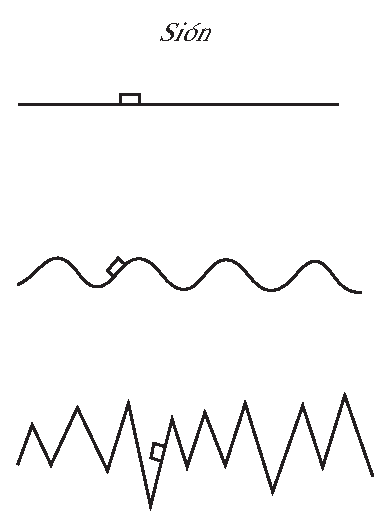
\includegraphics[width=6cm]{sion.eps}
\label{fig:sion}
\caption{La física cuántica sigue siendo hasta el día de hoy un fenómeno que no tiene una explicación concreta. Las ecuaciones vistas a lo largo de este curso describen la realidad y intentan darle sentido a algo que por ahí no fue diseñado para ser entendido en su totalidad. \emph{(Figura: Roberto Bolaño, 1998)}}
\end{figure}
\clearpage
%Anexo--------------------------------------------------->
%-------------------------------------------------------->
\part{Anexo}
%-----------------CONSTANTES
\section*{Constantes}
\begin{align*}
e&=\SI{1.602e-19}{\coulomb}\\
h&=\SI{6.626e-34}{\meter \squared \kg \per \second}\\
\boltz &=\SI{1.381e-23}{\meter \squared \kg \per \second \squared \per \kelvin }\\
b&=\SI{2.898e-3}{\meter \kelvin}\\
\sigma&=\SI{5.670e-8}{\watt \meter ^{-2} \kelvin ^{-4} }\\
m_p&=\SI{1.673e-27}{\kg}\\
    &=\SI{938.3}{\MeV/\lspeed ^2}\\
m_n&=\SI{1.675e-27}{\kg}\\
    &=\SI{939.6}{\MeV/\lspeed ^2}\\
m_e&=\SI{9.109e-31}{\kg}\\
    &=\SI{0.5110}{\MeV/\lspeed ^2}\\
m_{\pi^0}&=\SI{135.0}{\MeV/\lspeed ^2}\\
m_{\pi^{\pm}}&=\SI{139.6}{\MeV/\lspeed ^2}\\
m_{\mu}&=\SI{105.7}{\MeV/\lspeed ^2}\\
m_{\tau}&=\SI{1777}{\MeV/\lspeed ^2}\\
m_{\nu}&<\SI{0.120}{\eV/\lspeed ^2}\\
G  &=\SI{6.674e-11}{\meter \cubed \per \kilogram \per \second \squared}\\
\Lambda &= \SI{1.11e-52}{\per \meter \squared} \\
\Rydberg &=\SI{1.097e7}{\per \meter}  \\
\Avogadros &=\SI{6.02e23}{\atomos}\\
\SI{1}{amu}&=\SI{931.494}{\MeV/\lspeed^2}\\
\mu_B&=\SI{9.274e-24}{\joule \per \tesla}\\
&=\SI{5.788e-5}{\eV \per \tesla}\\
&=\SI{9.274e-21}{erg \per G}\\
\end{align*}

%-----------------TABLAS
\section*{Tablas}
\begin{table}[h]
\centering
\begin{tabular}{@{}lll@{}}
Clase & $\lambda$ & Energía \\ \hline
Radio & 1-10 \si{\meter} & 100-1000 \si{\nano \eV}  \\
Micro &1-100 \si{\mm}  & 1-1000\si{ \micro \eV} \\
Infrarrojo & 1-1000 \si{\micro\meter} &1-120 \si{\milli \eV}  \\
Visible & 400-700 \si{\nano \meter} &$\sim$ 1 \si{\eV} \\
UV &10-400 \si{\nano \meter} &3-100\si{\eV}  \\
Rx &100-1000 \si{\pico \meter} $\sim$ 1\si{\angstrom} &100-1000 \si{\eV}  \\ \bottomrule
\end{tabular}
\caption{Espectro electromagnético.}
\label{espectro}
\end{table}
%---------------OPERADORES
\section*{Operadores}
\begin{align*}
\hat{r}.[\;]&=r.[\;]\rightarrow \begin{cases}
\hat{x}=x \\
\hat{y}=y\\
\hat{z}=z
\end{cases} \\
\hat{p}_x.[\;]&=-i\hbar \spartial{[\;]}{x} \\
\hat{U}.[\;]&=U(\vec{r}).[\;]\\
\hat{E}.[\;]&=i\hbar \spartial{ }{t}\\
\hat{H}.[\;]&=-\frac{\hbar^2}{2m}\nabla^2[\;]+U(\vec{r}).[\;]\\
\hat{H}.[\;]&=  -\frac{\hbar^2}{2m}\frac{d^2[\;]}{dx^2}+U(x).[\;] \qquad \text{1 dimensión}\\
\hat{L}_z.[\;]&=\frac{\hbar}{i}\inpar{ x\spartial{[\;]}{y}-y\spartial{[\;]}{x} }\equiv \frac{\hbar}{i}\spartial{[\;]}{\varphi} \\
\hat{L}^2.[\;] &= -\hbar^2\Bigg[  \frac{1}{\sin\theta}\spartial{ }{\theta} \bigg( \sin\theta \spartial{[\;]}{\theta}\bigg)+\frac{1}{\sin^2\theta}\dpartial{[\;]}{\varphi}  \Bigg]\\
\hat{\vec{\mu}}.[\;]&=-\mu_B\frac{\hat{\vec{L}}}{\hbar}\\ 
\big[ \hat{A};\hat{B} \big].[\;]&=\hat{A}\big(\hat{B}.[\;]\big)-\hat{B}\big(\hat{A}.[\;]\big)\\
[\hat{L}_x;\hat{L}_y]&=i\hbar \hat{L}_z \\
[\hat{L}_y;\hat{L}_z]&=i\hbar \hat{L}_x \\
[\hat{L}_z;\hat{L}_x]&=i\hbar \hat{L}_y \\
\end{align*}



%----------------FIGURAS
\subsection*{Figuras}
\begin{figure}[htb!]
\centering
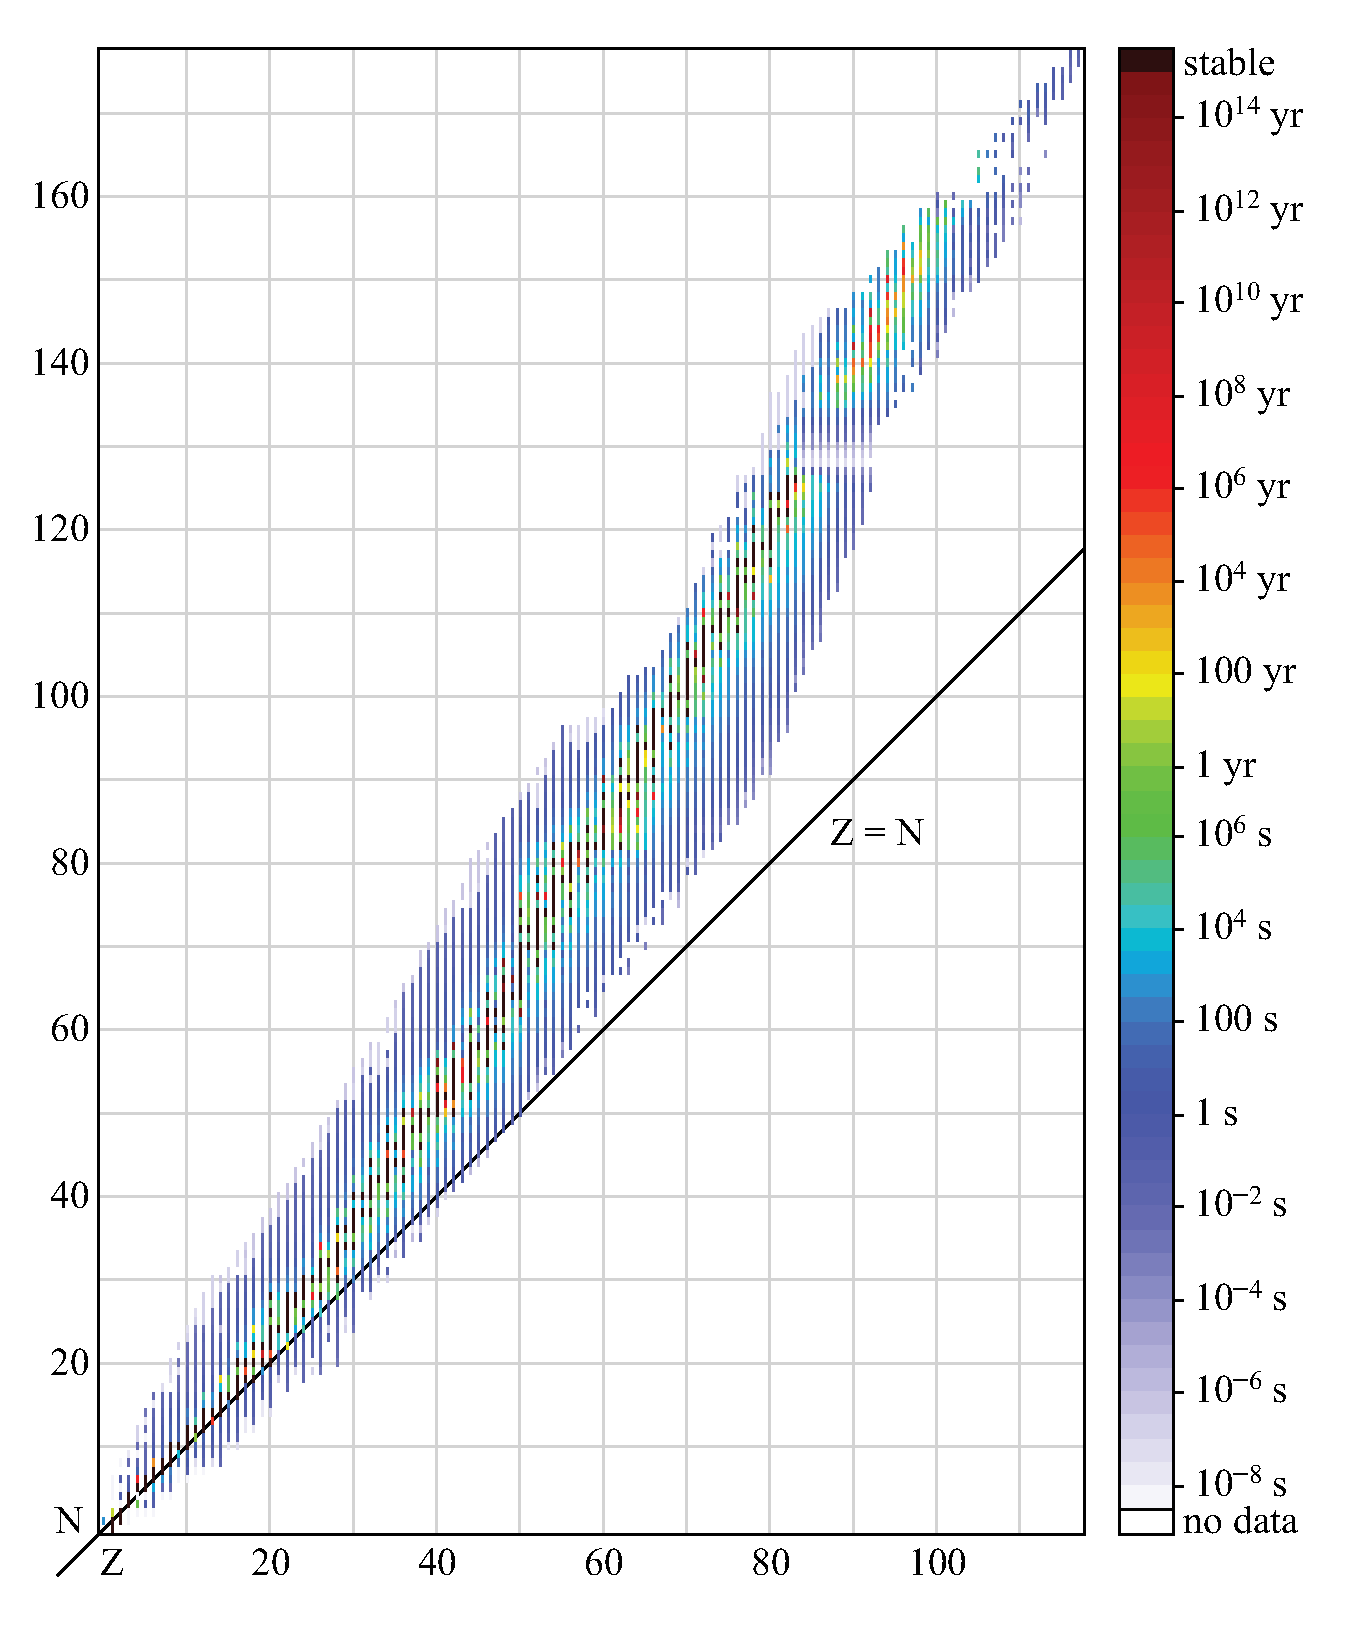
\includegraphics[width=7cm]{isotopos.eps}
\label{isotopos}
\caption{Estabilidad de los isotopos conocidos.}
\end{figure}

\end{document}
